% -*- root: main.tex -*-

\chapter{(De)composition of Homotopy Types}

We are now sufficiently armed both with an ample supply of algebraic invariants (e.g., homotopy groups) extracted from spaces, as well as two fundamental tools for forming new homotopy types: the exact and coexact extensions of a map of homotopy types.
In this Chapter, we turn to the following two questions of how these operations interact with respect to a designated homotopy type $X$:
\begin{enumerate}
    \item How can $X$ be constructed out of pieces with very simple invariants?
    \item How can $X$ be decomposed into pieces with simpler invariants?
\end{enumerate}
An attempt to understand the first question will lead us to the notion of a \define{CW--complex}, which is a particularly nice sort of space built out of homotopical data and coexact extensions.
An attempt to understand the second question will lead us to the notion of a \define{Postnikov tower}, which siphons off layers of a space into \define{Eilenberg--Mac Lane spaces} via exact extensions.
Ultimately, we will marry these two methods together to produce a concise tool for computing the collection of maps from one space to another, known as \define{obstruction theory}.




\section{CW complexes}

Our first framework for studying these kinds of questions is that of a \define{cell structure} on $X$.
Informally, such a structure is a kind of presentation of $X$ given by inductively ``attaching $n$--cells''.

\begin{definition}\marginnote{\citep[Definition 5.10]{Switzer}}
Consider a space $Y$ and a continuous map $g\co \bigvee_\alpha S^{n-1}_\alpha \to Y$.
We say that $Y \cup_g \bigvee_\alpha CS^{n-1}$ is \define{formed from $Y$ by attaching $n$--cells} (along $g$).
\end{definition}

\noindent
There are several motivations for considering this definition.
Mostly directly, it falls under the second heading: many commonly considered geometric spaces can be constructed by iteratively applying this operation.
Less directly, it also falls under the first heading: the homotopy class $g \in \pi_{n-1} Y$ is given an explicit null-homotopy in $Y \cup_g CS^{n-1}$, so that $g$ vanishes when pushed forward into $Y \cup_g CS^{n-1}$.

We here codify the entire inductive process that we mean:

\begin{definition}\marginnote{\citep[Definitions 5.1--3]{Switzer}}
We define a \define{CW--structure} on a space $X$ to be a choice of sequence of spaces $X_n$ satisfying certain properties.
The head of the bi-infinite sequence is fixed as $X^{-\infty} = \cdots = X^{-1} = \{x_0\}$.
Otherwise, $X^n$, called the \define{$n$--skeleton}, must be formed from $X^{n-1}$ by attaching $n$--cells.
Lastly, $X$ must be the union of the $X^n$ (with the weak topology).
\marginnote{If $A$ is a CW-complex, then setting $X^{-\infty} = \cdots = X^{-1} = A$ gives rise to a relative CW-structure $(X, A)$.}
If $X$ admits a CW--structure, then we say that it is a \define{CW--complex}.
\marginnote{%
Some topological facts about CW--complexes that might interest you:
\begin{itemize}
    \item Every CW--complex is Hausdorff.
    \item Every CW--complex is the disjoint union of the interiors of its cells.
    \item Each cell has only finitely many immediate faces.
    \item More generally, any compact subset has this property.
\end{itemize}
}
\end{definition}

\begin{example}\marginnote{\citep[Examples 5.4]{Switzer}}
Some common spaces come with the following natural CW--structures:
\begin{itemize}
    \item $S^n$ can be equipped with a CW--structure with only an $n$--cells, with boundary attached to the basepoint $\{x_0\}$.
    \todo{Picture}
    \item More elaborately, $S^n$ can be equipped with an inductive CW--structure: one can form $S^n$ from $S^{n-1}$ by attaching two $n$--cells, both along the identity map $S^{n-1} \to S^{n-1}$, which serve as the upper- and lower-hemispheres of $S^n$.
    \todo{Picture}
    \item The second collection of CW--structures are \define{compatible}, in the sense that the $m$--skeleton of $S^{n-1}$ agrees with the $m$--skeleton of $S^n$ for all $m < n$.  Using this, the union of these CW--structures puts a CW--structure on their colimit $S^\infty$.
    \item Each projective space $\RP^n$ (resp.\ $\CP^n$, $\HP^n$) can be endowed with a CW--structure where the $k$--skeleton is given by $\RP^k$ (resp.\ $\CP^k$, $\HP^k$), and one attaches $\R^n \cong CS^{n-1}$ (resp.\ $\C^n \cong CS^{2n-1}$, $\H^n \cong CS^{4n-1}$) along $\RP^{n-1}$ (resp.\ $\CP^{n-1}$, $\HP^{n-1}$) as the $0$\textsuperscript{th} affine chart to its complement.
    \item These CW--structures are also mutually compatible, so that one may form CW--structures on their respective colimits $\RP^\infty$, $\CP^\infty$, and $\HP^\infty$.
\end{itemize}
\end{example}

The inductive presentation means we can attack problems cell-by-cell.
For instance, we have the following simple applications of the gluing operation for topological spaces:
\begin{corollary}\marginnote{\citep[Proposition 5.5]{Switzer}}
Let $X$ be a space equipped with a CW--structure as above.
A function $f\co X \to Y$ is continuous if and only if the restriction \[\bigvee_n \bigvee_{\alpha \in A_n} CS^{n-1}_\alpha \to X \to Y\] to the ensemble of $n$--cells is continuous. \qed
\end{corollary}

\noindent
Since each $CS^{n-1}$ has a simple structure as a topological space, this is often an easier condition to manage.

It is also often possible to transfer CW--structures along other common topological operations.

\begin{lemma}\marginnote{\citep[pg.\ 71]{Switzer}}
If $X$ carries a CW--structure and $Y$ carries a \emph{finite} CW--structure, then $X \times Y$ carries an induced CW--structure.
\marginnote{If $X$ and $Y$ are infinite, then the weak topology on $X \times Y$ may not agree with the product of the weak topologies.  We mostly concede this point and pick the one we want (usually the former).}
\end{lemma}
\begin{proof}[Proof sketch]
Repeatedly use the homeomorphism $D^n \times D^m \cong D^{n+m}$.
\end{proof}

\begin{lemma}\marginnote{\citep[Exercise 5.14]{Switzer}}
If $X$ carries a CW--structure and $A \subseteq X$ is a subcomplex, then $X/A$ carries an induced CW--structure. \qed
\end{lemma}

\begin{corollary}\marginnote{\citep[Proposition 5.6]{Switzer}}
By consequence, homotopies and relative homotopies can also be constructed inductively over cells. \qed
\end{corollary}

These cell decompositions imbue maps from some common spaces with moduli-theoretic interpretations.

\begin{example}
The set of maps $S^n \to Y$ agrees with the set of maps $D^n \to Y$ which send $\partial D^n$ to $y_0$.
\end{example}

\begin{example}
Given $S^{n-1} \to Y$ and two choices of null-homotopies
\begin{center}
\begin{tikzcd}
S^{n-1} \arrow{d} \arrow{r} & Y \\
CS^{n-1} \arrow[shift left]{ru} \arrow[shift right]{ru},
\end{tikzcd}
\end{center}
we can form a difference class $S^n \to Y$.
Conversely, a map $S^n \to Y$ can be considered as the difference class associated to the null-homotopies of the restriction to the equator witnessed by the action of the map on two hemispheres.
\end{example}

\begin{example}
The space $\RP^2$ also participates in such a description.
Given a class $\omega\co S^1 \to Y$ and a null-homotopy of its double
\begin{center}
\begin{tikzcd}
S^1 \arrow["2\omega"]{r} \arrow{d} & Y \\
D^2 \arrow["H"]{ru},
\end{tikzcd}
\end{center}
we can form a map $\RP^2 \to Y$.
Conversely, a map $\RP^2 \to Y$ restricts to a class on $\RP^1$ whose double carries a specified null-homotopy.
\end{example}

We close out today by recording a technical topological result that will be absolutely crucial in underpinning the results in the next two Lectures.
Although we do not intend to offer careful proofs of those results, so that it is not \emph{necessary} to state this technical result either, we feel that a topology lecture would be remiss without it and that it gives some intuition as to why these nice results for CW--complexes are possible.

\begin{lemma}[Simplicial approximation]%
\marginnote{\citep[Proposition 6.8]{Switzer}}
Let $A$ be a CW--complex, and let $X = A \cup_g e^n$ consist of $A$ with a single $n$--cell attached.
Take $(K, L)$ to be a \emph{finite} simplicial pair, and consider a continuous map of pairs $f\co (|K|, |L|) \to (X, A)$.
There exists a subdivision $(K', L')$ of $(K, L)$ and a map $f'\co (|K'|, |L'|) \to (X, A)$ with the following properties:
\begin{enumerate}
    \item The two maps agree on $A$: \[f|_{f^{-1}(A)} = f'|_{f^{-1}(A)}.\]
    \item The two maps are homotopic while fixing their behavior on $A$: \[f \simeq_{\text{rel $f^{-1}(A)$}} f'.\]
    \item For each simplex $\sigma \in K'$, if $f'(|\sigma|)$ meets the interior $\overset \circ e^n$ of the new cell in $X$, then $f'(|\sigma|) \subseteq \overset \circ e^n$ is in fact contained in the new cell \emph{and} $f'|_{|\sigma|}$ restricted to this simplex is a linear map. \qed
\end{enumerate}
\end{lemma}





\section{The homotopy theory of CW complexes I}

In the previous section, we discussed CW--structures as placed on a preordained topological space $X$.
One can also take the perspective that the CW--structure is the primary data, and the colimit $X$ simply is whatever it is.
From this second viewpoint, the most important property of CW--complexes which makes them suitable for use in homotopy theory is that if the attaching maps $g$ are perturbed within their homotopy class to some $g' \sim g$, the resulting CW--complex $X'$ is homotopy equivalent to the original CW--complex $X$.
As ever, this is easiest to argue cell-by-cell.

\begin{lemma}
\todo{Find me a citation.}
Given two maps $g_1, g_2\co S^{n-1} \to A$, consider the associated cell complexes $X_1 = CS^{n=1} \cup_{g_1} A$ and $X_2 = CS^{n-1} \cup_{g_2} A$.
A homotopy $H\co g_1 \sim g_2$ begets a homotopy equivalence $X_1 \xrightarrow{\simeq} X_2$.
\end{lemma}
\begin{proof}[Construction] 
Subdivide $CS^{n-1}$ into an outer annulus (corresponding to the cone coordinate range $[1/2, 1]$) and an inner disk (corresponding to the cone coordinate range $[0, 1/2)$).
The homotopy equivalence is then given by gluing the identity map on $A$, the homotopy $H$ on the outer annulus, and the homeomorphism $S^{n-1} \sm [0, 1/2] \cong CS^{n-1}$ on the inner disk.
\end{proof}

This is the most basic property that one could ask of CW--complexes, but in fact they are remarkably well-behaved homotopically.  Our goal today is to get \emph{familiar}\marginnote{But not prove!} with some of these features and to use them to compute $\pi_{* \le n} S^n$.

\begin{lemma}%
\marginnote{\citep[Theorem 6.10]{Switzer}}
\marginnote{cf. \Cref{ConnectedDefn}}
For $(X, A)$ a relative CW-complex, the relative pair $(X, (X, A)^n)$ formed from the $n$--skeleton is $n$--connected. \qed
\end{lemma}

\begin{corollary}\label{XnIntoXIsNConnected}%
\marginnote{\citep[Theorem 6.11]{Switzer}}
The inclusion $X^n \to X$ is $n$--connected. \qed
\end{corollary}

\begin{corollary}\marginnote{\citep[Corollary 6.12]{Switzer}}
$\pi_{< n} S^n = 0$.
\end{corollary}
\begin{proof}
We deploy the cell structure on $S^n$ with $(S^n)^{n-1} = \{s_0\}$.
The long exact sequence of relative homotopy groups\marginnote{\Cref{LexseqOfRelativeHtpy}} takes the form \[\cdots \to \pi_k \{s_0\} \to \pi_k S^n \to \pi_k (S^n, \{s_0\}) \to \pi_{k-1} \{s_0\} \to \cdots.\]
The outer terms are always zero, as the homotopy groups of a singleton space.
The relative term $\pi_k (S^n, \{s_0\})$ vanishes for $k < n$, using \Cref{XnIntoXIsNConnected}.
Altogether, this shows the same of the non-relative groups $\pi_{<n} S^n$.
\end{proof}

\begin{lemma}\label{NConnectedSpacesHaveSmallModels}%
\marginnote{\citep[Proposition 6.13]{Switzer}}
If $(X, A)$ is $n$--connected, then there exists an equivalence $(X, A) \sim (X', A')$ with $(X', A')^n = A'$. \qed
\marginnote{This is a kind of converse to the previous Lemma.}
\marginnote{Taking $A = *$, this says that if $\pi_{< n} X = 0$, then there is a CW--model of $X$ with no cells below dimension $n$~\citep[Corollary 6.14]{Switzer}.}
\end{lemma}

\begin{corollary}\marginnote{\citep[Corollary 6.15]{Switzer}}
For $X$ an $n$--connected CW--complex and $Y$ an $m$--connected CW--complex, the CW--complex $X \sm Y$ is $(n+m+1)$--connected.
\end{corollary}
\begin{proof}
The cells in $X \times Y$ take the form $* \times *$, $* \times e_\beta^j$, $e_\alpha^i \times *$, and $e_\alpha^i \times e_\beta^j$.
All the first three classes lie within $X \vee Y$, so the first nontrivial surviving cell in $X \sm Y$ lies in dimension at least $n + m + 2$.
\todo{This cell structure argument also feeds into the claim that the suspension of a CW complex has predictable cell structure and predictable attaching maps.}
\end{proof}

\noindent Some of these miraculous properties again look like theorems we've previously seen for homology---but with a bound imposed, depending on the connectivities of the spaces involved.

\begin{theorem}[Homotopy excision]\label{HomotopyExcision}%
\marginnote{\citep[Theorem 6.21]{Switzer}}
Let $A, B \subseteq X$ be subspaces of $X$ such that $(A, A \cap B)$ is an $n$--connected pair and $(B, A \cap B)$ is an $m$--connected pair.
The natural double inclusion $\pi_*(A, A \cap B) \to \pi_*(X, B)$ is an isomorphism for $* < n+m$ and an epimorphism for $* = n+m$. \qed
\end{theorem}

\begin{corollary}\marginnote{\citep[Corollary 6.22]{Switzer}}
Suppose that $(X, A)$ is an $n$--connected pair and that $A$ is $m$--connected.
Then the natural map $\pi_*(X, A) \to \pi_* X/A$ is an isomorphism for $1 < * \le n+m$ and an epimorphism at $n+m+1$.
\end{corollary}
\begin{proof}
Consider the space $X \cup_A CA$, as well as the subspaces $CA$ and $X$ inside of it.
Noting that $CA \cap X = A$ as subspaces of $X \cup_A CA$, \Cref{HomotopyExcision} then gives the desired conclusion for the natural map \[\pi_*(X, A) \to \pi_*(X \cup_A CA, CA).\]
The right-hand group can be made non-relative by passing along the projection, as in \[(X \cup_A CA, CA) \xrightarrow\simeq (X \cup_A CA/CA, *).\]
\todo{There should be some Lemma recording that working relative to a contractible subspace is the same as quotienting out the subspace.
This is 6.6 in Switzer.}
To conclude, apply \Cref{ConeAndQuotIsRedundant} to produce a weak equivalence \[X/A \xrightarrow\simeq X \cup_A CA/CA. \qedhere\]
\end{proof}

\begin{corollary}[Freudenthal suspension theorem]\label{FreudenthalThm}%
\marginnote{\citep[Theorem 6.26]{Switzer}}
For an $n$--connected CW--complex $X$, the natural map
\marginnote{%
The left-hand vertical map is given by restriction to the boundary.
Its participation in the long exact sequence of relative homotopy groups shows it to be an equivalence, since $CX$ is contractible.
}
\begin{center}
\begin{tikzcd}
\pi_{*+1}(CX, X) \arrow{r} \arrow[equal]{d} & \pi_{*+1}(CX/X) \arrow[equal]{d} \\
\pi_* X \arrow{r} & \pi_{*+1} \Susp X
\end{tikzcd}
\end{center}
is an isomorphism for $* \le 2n$ and an epimorphism for $* = 2n+1$. \qed
\end{corollary}

\begin{example}\label{PinSnWithoutHurewicz}%
\marginnote{\citep[Theorem 6.28]{Switzer}}
Consider the following fibration:%
\marginnote{%
The top row presents this fibration as a fiber bundle.
To see that it is a fiber bundle, we rely on \Cref{GrassmanniansAreFiberBundles} and the sequence \[U(1) \to \frac{U(n)}{U(n-1)} \to \frac{U(n)}{U(n-1) \times U(1)}.\]
}
\begin{center}
\begin{tikzcd}
\C^\times \arrow{r} \arrow["\simeq"]{d} & \C^n \setminus 0 \arrow{r} \arrow["\simeq"]{d} & \CP^{n-1} \arrow["\simeq"]{d} \\
S^1 \arrow{r} & S^{2n-1} \arrow{r} & \CP^{n-1}.
\end{tikzcd}
\end{center}
Since $S^{2n-1}$ is $(2n-2)$--connected, we conclude $\pi_{*+1} \CP^{n-1} \cong \pi_* S^1$ for $* \le 2(n-1)$.
Using \Cref{Pi1S1Calculation}, we may conclude \[\pi_* \CP^n \cong \begin{cases} \Z & \text{when $* = 2$}, \\ 0 & \text{when $* < 2n-1$ and $* \ne 2$}, \\ ??? & \text{otherwise}. \end{cases}\]
We also know that $(\CP^{n-1}, \CP^1)$ is $2$--connected, from which we may conclude $\pi_2 \CP^1 \cong \pi_2 \CP^{n-1} \cong \pi_1 S^1 \cong \Z$, even though this is outside of the range directly accessible by the fibration alone.
This then feeds into Freudenthal as applied to the sphere, which for $n \ge 2$ gives \[\pi_n S^n \cong \pi_{n+1} S^{n+1}.\]
Hence, we ultimately conclude $\pi_n S^n \cong \Z$ for all $n \ge 1$.
\end{example}




\section{The homotopy theory of CW complexes II}

We continue our study of the pleasant homotopical properties of CW--complexes.
The following technical lemma appeared in our study of the relative homotopy long exact sequence of a pair $(Y, B)$:
\begin{lemma}\marginnote{\citep[Proposition 3.14]{Switzer}}
\todo{Backreference.}
For all solid squares
\begin{center}
\begin{tikzcd}
B \arrow{r} & Y \\
S^{n-1} \arrow["\omega|_{S^{n-1}}"]{u} \arrow{r} & D^n \arrow["\omega"]{u} \arrow[densely dotted, "\omega'"]{lu}
\end{tikzcd}
\end{center}
there exists a dashed filler for which the top-right triangle commutes up to homotopy. \qed
\todo{Add a $2$--cell from $Y$ to filler arrow.}
\end{lemma}

\noindent
This can be augmented in two ways: first, by extending it to cover more complicated sub-complexes, and second, by using it to govern the behavior of maps.

\begin{lemma}\label{NEquivsLiftNDimlSources}%
\marginnote{\citep[Theorem 6.30]{Switzer}}
If $f\co Z \to Y$ is an $n$--equivalence and $\dim(X, A) \le n$, then for each solid square
\begin{center}
\begin{tikzcd}
Z \arrow["f"]{r} & Y \\
A \arrow["g"]{u} \arrow{r} & X \arrow["h"]{u} \arrow[densely dotted]{lu}
\end{tikzcd}
\end{center}
there exists a dashed filler such that the top-right triangle commutes up to homotopy. \qed
\todo{Add a $2$--cell from $Y$ to filler arrow.}
\end{lemma}

\begin{corollary}\marginnote{\citep[Theorem 6.31]{Switzer}}
Given an $n$--equivalence $f\co Z \to Y$ and a CW--complex $X$ of dimension at most $n$, the natural map \[f_*\co [X, Z] \to [X, Y]\] is surjective.
If the dimension of $X$ is exactly $n$, $f_*$ is an isomorphism.
\qed
\end{corollary}

\noindent
These results ultimately culminate in the following:

\begin{corollary}[Whitehead]\marginnote{\citep[Theorem 6.32]{Switzer}}
A weak equivalence $f\co Z \to Y$ of CW-complexes is a homotopy equivalence.
\qed
\end{corollary}

\noindent
Here, finally, is justification that relative homotopy groups truly do measure the discrepancy between two spaces:
\marginnote{Provided that those spaces are sufficiently nice!}
if the discrepancy vanishes, then the two spaces are equivalent in the homotopy category.

Filtering a CW-complex by its skeleta and applying the Lemma yields the second thread of useful results.

\begin{definition}\marginnote{\citep[Definition 6.34]{Switzer}}
A map $f\co X \to Y$ of CW--complexes $X$ and $Y$ is said to be \define{cellular} if it carries the $k$\textsuperscript{th} skeleton of $X$ to the $k$\textsuperscript{th} skeleton of $Y$: \[f(X^k) \subseteq Y^k.\]
\end{definition}

\begin{corollary}\marginnote{\citep[Proposition 6.35]{Switzer}}
Every map $f\co (X, A) \to (Y, B)$ of CW-complexes is homotopic (relative to $A$) to a cellular map, and homotopies between cellular maps admit cellular replacements. \qed
\end{corollary}

Together, these results grant us serious control over how the homotopy groups of a CW--complex change as its skeleta are built up---in the qualitative sense of \emph{which} groups change.
This can be deployed to manufacture certain interesting spaces, called Eilenberg--Mac Lane spaces, which we spend the rest of today doing.

\begin{corollary}\marginnote{\citep[Proposition 6.36]{Switzer}}
Let $X$ be an $n$--connected CW--complex, and let $Y$ be an $m$--connected CW--complex.
The natural map $X \vee Y \to X \times Y$ induces an isomorphism in homotopy through a range: \[\pi_{\le n+m}(X \vee Y) \xrightarrow\cong \pi_{\le n+m}(X \times Y)\]
\end{corollary}
\begin{proof}
Last time, we argued that the cellular structure induced on $X \times Y$ was completely contained in $X \vee Y$ through a range: \[(X \times Y, X \vee Y)^{n+m+1} = (X \vee Y)^{n+m+1}.\]
The relative homotopy groups of the pair thus vanish through this range, and the long exact sequence yields the desired statement.
\end{proof}

\begin{corollary}\label{PinOfSphereBouquet}%
\marginnote{\citep[Corollary 6.37]{Switzer}}
For $n \ge 2$,
\marginnote{Also, $\pi_1 \bigvee_\alpha S^1_\alpha \cong \bigast_\alpha \pi_1 S^1_\alpha$.}
\[\pi_n\left(\bigvee_\alpha S^n_\alpha\right) \cong \bigoplus_\alpha \pi_n S^n_\alpha.
\qed\]
\end{corollary}

\begin{lemma}\marginnote{\citep[Theorem 6.39.i]{Switzer}}\label{EMSpacesExist}
For any abelian group $A$ and index $n \ge 2$, there exists a CW--complex $K(A, n)$ whose homotopy groups satisfy \[\pi_* K(A, n) = \begin{cases} A & \text{if $* = n$}, \\ 0 & \text{otherwise}. \end{cases}\]
\end{lemma}
\begin{proof}
Select a presentation \[0 \to \Z^J \xrightarrow g \Z^I \to A \to 0.\]
\todo{Explain one of the preceding results as saying that coexact sequences of spaces behave like exact sequences through a range.}
We intend to build a coexact sequence of $(n-1)$--connected spaces whose behavior on $\pi_n$ encodes the chosen presentation.
Begin by modeling the middle node as $\bigvee_I S^n$.
Combining \Cref{PinSnWithoutHurewicz} and \Cref{PinOfSphereBouquet} gives \[\pi_n\left( \bigvee_I S^n\right) \cong \bigoplus_I \Z.\]
The $J$--sized set of elements selected by $g$ gives a $J$--sized set of maps $S^n \to \bigvee_I S^n$, and hence a single map $\widetilde g\co \bigvee_J S^n \to \bigvee_I S^n$ which induces $g$ on $\pi_n$.
The cone on $g$ gives a complex $X_n$ with $\pi_{* < n} X_n = 0$ and $\pi_n X_n = A$.
\marginnote{We're not there yet, but $X_n$ is sometimes called a \define{Moore space} (of dimension $n$, for the group $A$), because $H_n(X_n; \Z) \cong A$.}
We inductively form $X_{n+j+1}$ from $X_{n+j}$ by killing the homotopy in degree $n+j+1$ by coning off any homotopy classes we find.
Using the long exact sequence of a relative pair, we see that this coning operation never disturbs the homotopy groups at or below $n+j$, so the colimit indeed provides $K(A, n)$.
\end{proof}

\begin{lemma}\label{ConnToCoconnIsAlgebraic}%
\marginnote{\citep[Theorem 6.39.ii]{Switzer}}
Let $X$ be a space satisfying $\pi_{< n} X = 0$, and let $Y$ be a space satisfying $\pi_{> n} Y = 0$.
\marginnote{$X$ is sometimes said to be \define{$n$--connective} and $Y$ to be \define{$n$--coconnective}.}
Then homotopy classes $[X, Y]$ biject with homomorphisms $\pi_n X \to \pi_n Y$.
\end{lemma}
\begin{proof}
Using \Cref{NConnectedSpacesHaveSmallModels}, there exists a CW model of $X$ with $X^{n-1} = *$.
The rest of the presentation of $X$ looks like:
\begin{center}
\begin{tikzcd}
\bigvee_I S^n \arrow[equal]{r} & X^n \arrow{r} & X^{n+1} \arrow{r} & X^{n+2} \arrow{r} & \cdots \arrow{r} & X \\
& \bigvee_J S^n \arrow{u} & \bigvee S^{n+1} \arrow{u} & \bigvee S^{n+2} \arrow{u} & \cdots \arrow{u}.
\end{tikzcd}
\end{center}
Using this presentation, we can inductively study the available maps into $Y$.
We begin with \[[X^n, Y] = \left[\bigvee_I S^n, Y\right] = \bigoplus_I \pi_n Y.\]
To extend along the $(n+1)$--skeleton, the precomposite \[\bigvee_J S^n \to \bigvee_I S^n \to Y\] must vanish, and the unicity of each such extension is measured by $[\Susp \bigvee_J S^n, Y] = 0$, so that we have an exact sequence
\begin{center}
\begin{tikzcd}
{[X^{n+1}, Y]} \arrow{r} \arrow[equal]{d} & {[X^n, Y]} \arrow{r} \arrow[equal]{d} & \left[\bigvee_J S^n, Y\right] \arrow[equal]{d} \\
\CatOf{Groups}(\pi_n X, \pi_n Y) \arrow{r} & \bigoplus_I \pi_n Y \arrow{r} & \bigoplus_J \pi_n Y.
\end{tikzcd}
\end{center}
\marginnote{%
For a generic CW--complex $Y$, without assumptions on its $\pi_{>n}$, the relative group $\pi_n(Y^n, Y^{n-1})$ is free on generators $\gamma \cdot [f^n_\alpha]$, where $\gamma \in \pi_1 X^{n-1}$, and $f^n_\alpha$ is the characteristic map of an $n$--cell.
}
For all higher stages, both the obstruction to extension vanishes (because $\pi_{n+k} Y = 0$) in addition to the unicity (because $\pi_{n+k+1} Y = 0$).
\end{proof}

\begin{corollary}\marginnote{\citep[Corollary 6.42]{Switzer}}
$K(A, n)$ is independent of choice of presentation.
\end{corollary}
\begin{proof}
Consider two models $X$, $Y$ for $K(A, n)$.
Both $X$ and $Y$ satisfy the conditions of the Lemma, so that the identity map $\id\co A \to A$ lifts to a map $\widetilde{\id}\co X \to Y$.
This map $\widetilde{\id}$ of CW--complexes is an isomorphism on homotopy groups, hence Whitehead's theorem witnesses it as a homotopy equivalence.
\end{proof}

\begin{remark}\label{ShiftingEMSpaces}\marginnote{\citep[Remark 6.45]{Switzer}}
Using \Cref{LoopsShiftsPi}, we may conclude that $\Loops K(A, n)$ has the same homotopy groups as $K(A, n-1)$.
The Corollary shows that it, in fact, does model $K(A, n-1)$ via a map \[\Loops K(A, n) \xrightarrow\simeq K(A, n-1).\]
However, the adjoint map $\Susp K(A, n-1) \to K(A, n)$ is more mysterious.
It can be taken to be an inclusion on $(n+1)$--skeleta, but otherwise it appears little can be said about it at this point.
We will meet it again.
\end{remark}

\begin{remark}\marginnote{\citep[Exercise 6.49]{Switzer}}
For \emph{all} spaces $X$, there exists a CW-complex $\widetilde X \to X$ such that the map is a weak equivalence.
\todo{This might be out of place. Trying to justify it probably reveals where it belongs.}
\end{remark}




\section{Spectral sequences}\label{SpectralSequenceSection}
\marginnote{
Our treatment here deviates from Switzer's, which can be found on~\citep[pg.\ 336--340]{Switzer}.
Our approach is closer to that of Boardman~\citep{Boardman}, though he is much more technically intense (and, of course, more rigorous).
}

The argument we gave in the proof of \Cref{ConnToCoconnIsAlgebraic} felt quite serendipitous and fragile.
Had our hypotheses been even slightly weaker, we would have quickly found it very difficult to keep track of all the interacting groups involved.
However, this kind of scenario is extremely common, where a space $X$ of interest is constructed from an infinite sequence of steps
\marginnote{As with cells in a CW--complex.}
and where we hope to compute some invariant, like $\pi_*(X)$, from knowledge of the relative invariants, like $\pi_*(X_n, X_{n-1})$.
It is so common, in fact, that topologists have worked to codify the formal properties of this scenario, which goes by the name of a \define{spectral sequence}.
Today we recount a mild specialization of this framework that will suit us well.
\marginnote{%
More generally, one might discuss \define{exact couples}.
}

We begin by arranging into a single diagram the exact sequences associated to each inclusion:

\begin{figure*}[h]
\begin{center}
\begin{tikzcd}[column sep=1em]
0 \arrow{r} & \pi_* X_1 \arrow{r} & \pi_* X_2 \arrow{r} \arrow{dl} & \cdots \arrow{r} \arrow{dl} & \pi_* X_n \arrow{r} \arrow{dl} & \pi_* X_{n+1} \arrow{r} \arrow{dl} & \cdots \arrow{r} \arrow{dl} & \pi_* X \\
& \pi_*(X_2, X_1) \arrow[red]{u} & \pi_*(X_3, X_2) \arrow[red]{u} & \cdots \arrow[red]{u} & \pi_*(X_{n+1}, X_n) \arrow[red]{u} & \pi_*(X_{n+2}, X_{n+1}) \arrow[red]{u} & \cdots,
\end{tikzcd}
\end{center}
\end{figure*}

\noindent
where each triangle is a ``rolled up'' exact sequence and each red arrow shifts degree by one, e.g., $\pi_*(X_{n+1}, X_n) \to \pi_{*-1} X_n$.
Let us study in earnest the problem of recovering $\pi_* X$ only by probing information about the groups $\pi_*(X_{n+1}, X_n)$ on the bottom row.
\marginnote{If we permitted ourselves access to the top row of $\pi_* X_n$, we could take a colimit and be done.}
Our first observation is that since each sphere is compact, every class $x \in \pi_* X$ must lift to some $\widetilde x \in \pi_* X_n$.
However, since this is not a relative group, we are not permitted to make direct use of it, and we should instead consider the image of this class $x_n \in \pi_*(X_n, X_{n-1})$ in the bottom row.
Our second observation is that at exactly the \emph{minimal} such $n$ to which (a nonzero class) $x$ lifts to $\widetilde x \in \pi_* X_n$, it pushes down to give a nonzero class $x_n \in \pi_*(X_n, X_{n-1})$.
This explains some of the classes in $\pi_*(X_n, X_{n-1})$.
How can we discern the classes that come from these minimal preimages?
What use are those classes that don't?

Let us thus begin from the other vantage point by selecting a class $x_n \in \pi_*(X_n, X_{n-1})$ and asking when there is a class $\widetilde x \in \pi_* X_n$ of which it is the image.

\begin{center}
\begin{tikzcd}
& & \textcolor{red}{\partial(x_n)} \arrow[red, |->]{lddd} & \textcolor{red}{(\exists \; \widetilde{x}???)} \arrow[red, densely dotted, |->]{lddd} \\
\cdots \arrow{r} & \pi_* X_{n-1} \arrow{r} & \pi_* X_n \arrow{r} \arrow{dl} & \pi_* X_{n+1} \arrow{r} \arrow{dl} & \cdots \\
& \pi_*(X_n, X_{n-1}) \arrow{u} & \pi_*(X_{n+1}, X_n) \arrow{u} & \pi_*(X_{n+2}, X_{n+1}) \arrow{u} \\
& \textcolor{red}{d_1(x_n)} & \textcolor{red}{x_n} \arrow[red, |->, bend left]{uuu}
\end{tikzcd}
\end{center}

From $x_n$, we can manufacture two more classes: $\partial(x_n) \in \pi_* X_n$ and $d_1(x_n) \in \pi_*(X_n, X_{n-1})$.
The existence of $\widetilde x$ is determined by whether $\partial(x_n)$ is nonzero---but, since it is not on the bottom row, we cannot ask about it directly.
We are allowed to probe $d_1(x_n)$ directly.
If it is not zero, then surely $\partial(x_n)$ is also not zero, which settles the question definitively that a lift $\widetilde{x}$ cannot exist.
On the other hand, if it is zero, then it could be the case that $\partial(x_n)$ is zero (so that $\widetilde{x}$ exists) or that $\partial(x_n)$ is nonzero and merely in the kernel of the map $\pi_* X_n \to \pi_*(X_n, X_{n-1})$.
In the second case, we can use exactness to build a preimage $i_n^{-1} \partial(x_n) \in \pi_* X_{n-1}$, as in:

\begin{figure*}[h]
\begin{center}
\begin{tikzcd}
& & \textcolor{red}{i_n^{-1} \partial(x_n)} \arrow[red,|->]{r} \arrow[red,|->]{lddd} & \textcolor{red}{\partial(x_n)} \arrow[red, |->]{lddd} & \textcolor{red}{(\exists \; \widetilde{x}???)} \arrow[red, densely dotted, |->]{lddd} \\
\cdots \arrow{r} & \pi_* X_{n-2} \arrow{r} & \pi_* X_{n-1} \arrow{r} & \pi_* X_n \arrow{r} \arrow{dl} & \pi_* X_{n+1} \arrow{r} \arrow{dl} & \cdots \\
& \pi_*(X_{n-1}, X_{n-2}) \arrow{u} & \pi_*(X_n, X_{n-1}) \arrow{u} & \pi_*(X_{n+1}, X_n) \arrow{u} & \pi_*(X_{n+2}, X_{n+1}) \arrow{u} \\
& \textcolor{red}{d_2(x_n)} & \textcolor{red}{0} & \textcolor{red}{x_n} \arrow[red, |->, bend left]{uuu}
\end{tikzcd}
\end{center}
\end{figure*}

We make a series of claims:
\begin{enumerate}
    \item This assignment $d_2$ is well-defined up to the image of $d_1$, and hence it determines a function $d_2\co H_*(\pi_*(X_*, X_{*-1}); d_1) \to H_{*-1}(\pi_*(X_{*-2}, X_{*-3}); d_1)$.
    \item This process continues step-by-step exactly as written.  Since $X_0 = *$, eventually the preimage is guaranteed to be zero, hence $\partial(x_n) = 0$, and hence $\widetilde x$ exists.
    \item The surviving elements in a spectral sequence are the associated graded of a filtration of $\pi_* X$ (by minimal lift degree).
\end{enumerate}
\todo{Introduce some terminology, especially \define{pages}.}

\begin{remark}
This story can be retold with many variations.
Some introduce no further complexity:
\begin{itemize}
    \item In place of exact sequences of spaces and relative homotopy groups, one can use coexact sequences of spaces and a homology functor.
    \todo{Are there other simple variants?}
\end{itemize}
Others introduce substantial complexity:
\begin{itemize}
    \item The filtration can be bi-infinite, dropping the assumption that $X_0 = *$.
    \item The spectral sequence can be ``infinite to the left'' (e.g., when applying a \emph{cohomology} functor to a filtration by coexact sequences).
    \item If one does not introduce assumptions to avoid this, since homotopy groups of low orders are not abelian groups, their homological algebra is substantially more complicated (especially when coupled to the above variants).
\end{itemize}
The essential complexity introduced by the first two points is that such spectral sequences need not \emph{stabilize}.
In order to handle this, one has to incorporate taking inverse limits of the subquotients of $H_* A_*$, which can destroy some of the exactness in the third Claim or the argument used to justify the second Claim.
\end{remark}

Spectral sequences have the simultaneous pleasant features of being valuable computational tools while also being sufficiently rigid that one can use them to prove theorems without computing anything.
The following result is an example of their rigidity:

\begin{lemma}
A \define{map of spectral sequences} is a family of homomorphisms from the ``bottom row'' of one to the ``bottom row'' of the other which additionally commute with all of the $d_r$ maps.
If a map of spectral sequences is an isomorphism on the $r$\textsuperscript{th} page for any $r$, it is an isomorphism forever after.
Their targets are also isomorphic by the same map. \qed
\end{lemma}

\begin{example}\label{CellularHomologyWorks}
Consider the filtration of a CW-complex $X$ by its skeleta.
The filtration stages participate in coexact sequences with spheres of a fixed dimension, from which we conclude \[\widetilde H_*(X_n, X_{n-1}; A) = \widetilde H_*\left(\bigvee_\alpha S^n_\alpha ; A\right) = \bigoplus_\alpha \Susp^n A.\]
The map $d_1$ associated to the spectral sequence is exactly the cellular differential, as can be seen by drawing the defining diagram:
\begin{center}
\begin{tikzcd}
\widetilde H_* X_{n_1} \arrow{r} & \widetilde H_* X_n \arrow{ld} \\
\widetilde H_* \bigvee_\beta S^{n-1}_\beta \arrow{u} & \widetilde H_* \bigvee_\alpha S^n_\alpha \arrow{u} \arrow["d_1"]{l}.
\end{tikzcd}
\end{center}
It follows that the $E_2$--page is given by $H_*(H_*(X_*, X_{*-1}); d_1) = \widetilde H_*^{\mathrm{cell}}(X; A)$.
All higher differentials are zero because \[d_r\co \bigoplus_\alpha \Susp^n A \xrightarrow{[-1]} \bigoplus_\gamma \Susp^{n-r} A\] has the wrong degree.
We say that the spectral sequence \define{collapses at $E_2$}, and this is a proof of that cellular homology computes homology.
\end{example}

\begin{corollary}\label{SpheresDetectEquivalenceOfCohomologyTheories}
More genrally, if $E$ and $F$ satisfy Eilenberg--Steenrod and $E_*(S^n) \to F_*(S^n)$ is an isomorphism for all $n$, then $E_*(X) \to F_*(X)$ is an isomorphism for all CW complexes $X$. \qed
\end{corollary}

\begin{example}\label{EMSpacesRepresentOrdinaryCoh}
The Eilenberg--Mac Lane spaces play another important role in homotopy theory which we will more seriously explore in \Cref{RepChap}.
Fixing an abelian group $A$ and letting $n$ vary, the functors \[X \mapsto [X, K(A, n)]\] satisfy the Eilenberg--Steenrod axioms: they carry wedge sums to products, and they convert coexact sequences of spaces to long exact sequences of groups.
Moreover, there is a natural transformation
\begin{align*}
{[X, K(A, n)]} & \to H^n(X; A), \\
f & \mapsto f^* \iota_n,
\end{align*}
where $\iota_n \in H^n(K(A, n); A)$ represents the identity map \[H_n(K(A, n); \Z) \cong A \xrightarrow{\id} A.\]
It then follows from \Cref{SpheresDetectEquivalenceOfCohomologyTheories} that this natural transformation is actually a natural \emph{isomorphism}.
\end{example}




\section{Obstruction theory}\label{ObstructionSection}

Today we exploit the machinery of spectral sequences to organize and extend some of our results in the realm of \define{obstruction theory}.
Obstruction theory is generally concerned with starting with a map
\begin{center}
\begin{tikzcd}
A \arrow{r} & B
\end{tikzcd}
\end{center}
and extending it to a diagram of the form
\begin{center}
\begin{tikzcd}
A \arrow{r} \arrow{d} \arrow[densely dotted]{rd} & B \\
X \arrow[densely dotted]{r} \arrow[densely dotted]{ru} & Y \arrow{u}
\end{tikzcd}
\end{center}
where any one of the dashed maps might be the goal.
We will focus our efforts by setting $A = B = *$, so that we will equivalently describe a method to compute $\pi_0 Y^X$ from the data of $X$ and of $Y$ separately.
\marginnote{The ``relative'' cases where $A$ and $B$ are nonzero we leave to the interested reader.}

Recall one the following Lemma from our study of the homotopy-theoretical properties of CW--complexes:
\begin{lemma}\marginnote{\Cref{ConnToCoconnIsAlgebraic}}
For $Y$ an $n$--connective CW--complex and $Z$ an $n$--coconnective CW--complex,
\marginnote{Recall that $n$--connective is a synonym for $(n-1)$--connected, and $n$--coconnective for $\pi_{>n} Z = 0$.}
the natural map $[Y, Z] \to \CatOf{Groups}(\pi_n Y, \pi_n Z)$ is an isomorphism. \qed
\end{lemma}

\noindent
This Lemma falls squarely into the realm of obstruction theory: it gives an algebraic description of what maps between certain homotopy types exist.
Its proof also relied on spectral-sequence-style machinery, so it seems ripe for us to generalize now.

In the moment, however, we only needed the Lemma as part of a program to construct and analyze certain spaces called $K(A, n)$.
It was the key ingredient in showing that the presentation of $A$ used in their construction was purely auxiliary, and that $K(A, n)$ itself was a well-defined object.
It has another application: the construction of \define{Postnikov towers}.

\begin{corollary}
If $Y$ is $n$--connective, then there is a canonical map \[Y \to K(\pi_n Y, n)\] induced by the identity on $\pi_n$. \qed
\end{corollary}

\begin{corollary}\label{PostnikovTruncationsExist}
For $Y$ an $n$--connective space, the exact extension of the canonical map $Y \to K(\pi_n Y, n)$ is called the \define{$(n+1)$--upward-truncation of $Y$}, denoted $Y(n, \infty)$ or $Y[n+1, \infty)$.
It has the properties \[\pi_* Y(n, \infty) = \begin{cases} \pi_* Y & \text{if $* > n$}, \\ 0 & \text{otherwise} \end{cases}\] and $\pi_* Y(n, \infty) \to \pi_* Y$ is an isomorphism for $* > n$.
\marginnote{In fact, it is the universal $n$--connected space over $Y$: any map in from any other such $n$--connected space factors through $Y(n, \infty)$.}
\end{corollary}
\begin{proof}
This is entirely an application of the long exact sequence of relative homotopy.
\end{proof}

\begin{definition}
Starting with a $0$--connected space and repeatedly applying \Cref{PostnikovTruncationsExist} leads to the \define{Postnikov tower},

\begin{figure*}[h]
\begin{center}
\begin{tikzcd}
Y \arrow{d} & Y(1, \infty) \arrow{l} \arrow{d} & Y(2, \infty) \arrow{l} \arrow{d} & \cdots \arrow{l} & Y(n, \infty) \arrow{l} \arrow{d} & \cdots \arrow{l} & * \arrow{l} \\
K(\pi_1 Y, 1) & K(\pi_2 Y, 2) & K(\pi_3 Y, 3) & & K(\pi_{n+1} Y, n+1),
\end{tikzcd}
\end{center}
\end{figure*}

which is a diagram of interlocking exact sequences.
\end{definition}

This situation is ripe for a spectral sequence.
\marginnote{Simply applying $\pi_*$ to this diagram gives an extremely boring spectral sequence!}
We apply $\pi_* F(X, -)$, where $X$ is some fixed test space.  The functor $F(X, -)$ preserves exact sequences, $\pi_*$ turns them into long exact sequences, and \Cref{EMSpacesRepresentOrdinaryCoh} shows that $\pi_* F(X, K(\pi_{n+1} Y, n+1))$ has a recognizable form.
Bundling these results together gives:

\begin{definition}\label{FedererSSeq}
\define{Federer's spectral sequence} has signature
\marginnote{%
As previously remarked, for arbitrary $X$ and $Y$ the objects $\pi_0$ and $\pi_1$ of $F(X, Y)$ are \emph{sets} and \emph{groups} respectively.
This situation is called a \define{fringed spectral sequence}, which is considerably more obnoxious.
Ensure $X = \Susp^2 X'$ or $Y = \Loops^2 Y'$ for an easy way to avoid this situation.
}
\begin{align*}
E^1_{m, n} & = \pi_m F(X, K(\pi_{n+1} Y, n+1)) \\
& = \widetilde H^{n-m+1}(X; \pi_{n+1} Y) \Rightarrow \pi_m F(X, Y).
\end{align*}
\end{definition}

\begin{remark}
If $\pi_{< n} X = 0$ and $\pi_{> n} Y = 0$, we have $H^{< n}(X; \text{any}) = 0$ and $H^{\text{any}}(X; \pi_{> n} Y) = 0$.
This puts a single nonvanishing group in the region of the spectral sequence contributing to $\pi_0 Y^X$: \[H^n(X; \pi_n Y) \cong \CatOf{AbGps}(H_n X, \pi_n Y) \cong \CatOf{AbGps}(\pi_n X, \pi_n Y).\]
Since this group cannot be the source or target of any differentials, we conclude \Cref{ConnToCoconnIsAlgebraic}: \[\CatOf{AbGps}(\pi_n X, \pi_n Y) \cong F(X, Y).\]
\end{remark}

\begin{corollary}\label{OrdinaryCohIsRepresentable}
Ordinary cohomology is representable: \[\widetilde H^n(X; A) \cong [X, K(A, n)].\]
\end{corollary}
\begin{proof}
Take $Y = K(A, n)$ in \Cref{FedererSSeq}.
The spectral sequences collapses to give \[\pi_m F(X, K(A, n)) \cong \widetilde H^{n-m}(X; A). \qedhere\]
\end{proof}

\begin{remark}
The relative version of this spectral sequence also recovers \Cref{NEquivsLiftNDimlSources}.
\end{remark}

Even though we have constructed this very appealing machine, we must stop short of actually using it to do anything.
Nothing comes for free: the price of organizing the information in the $E_1$--term of a spectral sequence in a pretty way means that the differentials will surely be difficult to understand.
To see what can happen, consider the $d_1$--differential, which is induced by pushforward along the map $k_n$ in
\begin{center}
\begin{tikzcd}
Y[n, \infty) \arrow{dd} & & Y(n, \infty) \arrow{ll} \arrow{dd} \\
& \Loops K(\pi_n Y, n) \arrow{ru} \arrow[red, bend left, "k_n"]{rd} \\
K(\pi_n Y, n) & & K(\pi_{n+1} Y, n+1).
\end{tikzcd}
\end{center}
This map is part of the homotopy data of $Y$ called the \define{$n$\textsuperscript{th} $k$--invariant} of $Y$.
\marginnote{Indeed, it appears naturally when constructing $Y = X^{S^0}$ from $S^0$ using obstruction theory.  Also, the ``$k$'' is presumably the same ``$K$'' appearing in ``$K(A, n)$''.}
As noted in \Cref{ShiftingEMSpaces}, we have a weak equivalence \[\Loops K(\pi_n Y, n) \simeq K(\pi_n Y, n-1),\] so that $k_n$ can be considered as a map of Eilenberg--Mac Lane spaces: \[k_n\co K(\pi_n Y, n-1) \to K(\pi_{n+1} Y, n+1).\]
This induces a natural transformation
\begin{center}
\begin{tikzcd}
{[-, K(\pi_n Y, n-1)]} \arrow["(k_n)_*"]{r} \arrow[equal]{d} & {[-, K(\pi_{n+1} Y, n+1)]} \arrow[equal]{d} \\
H^{n-1}(-; \pi_n Y) \arrow{r} & H^{n+1}(-; \pi_{n+1} Y).
\end{tikzcd}
\end{center}
This leaves us with some burning questions which we must answer before using this spectral sequence with any seriousness:
\begin{enumerate}
    \item What do natural transformations of the cohomology functor look like in general? How many are there? Is there a classification, or a general formula?
    \marginnote{This is kind of the ``dual problem'' to trying to compute $[S^m, S^n]$.}
    \item How can they be discerned / extracted for some space $Y$?
\end{enumerate}




\begin{subappendices}
\section{A complicated example}\label{ComplicatedExampleSec}

We haven't yet had an example of a spectral sequence in which we can compute.
This is because at our stage it is impossible to find a spectral sequence that is easy, tangible, nontrivial, and well-motivated all at once.
Today we will retreat to algebra in order to work an example that covers the first three attributes, with the promise that it will become well-motivated later on.

Let us consider the Hopf algebra \[\A(1)_* = \F_2[\xi_1, \xi_2] / (\xi_1^4, \xi_2^2)\] whose comultiplication is determined by%
\marginnote{%
Topologists often write ``$\mid$'' in place of ``$\otimes$'' to make lengthy formulas less exhausting to write.
This practice is also where the name ``co/\emph{bar} complex'' comes from.
}
\begin{align*}
\Delta \xi_1 & = 1 \mid \xi_1 + \xi_1 \mid 1, \\
\Delta \xi_2 & = 1 \mid \xi_2 + \xi_1 \mid \xi_1^2 + \xi_2 \mid 1.
\end{align*}
Associated to this Hopf algebra there is a \define{(reduced) cobar complex}, given by \[C^n(\A(1)_*) = \left\{\cdots \to \overline \A(1)^{\otimes n} \xrightarrow{\delta^n} \overline \A(1)^{\otimes (n+1)} \to \cdots \right\},\] where $\overline{\A(1)}$ denotes the quotient of $\A(1)$ by the submodule spanned by the unit class.
The differential $\delta^n$ is given by the alternating sum \[\delta^n(x_1 \mid \cdots \mid x_n) = \sum_{j=1}^n (-1)^{j+1} \left(x_1 \mid \cdots \mid \Delta(x_j) \mid \cdots \mid x_n\right).\]

\todo{Credit Reuben Stern for these beautiful pictures!}
Despite being only of modest size, the cohomology of this complex is still fairly difficult to compute.
Before turning spectral sequences to bear on this problem, we use the theory of derived functors to perform a manual computation, so that the reader has a firmer sense of the effort that is being saved.
The subalgebra $\A(1) \subset \A$ can be represented pictorially as in the margin.
\marginnote{
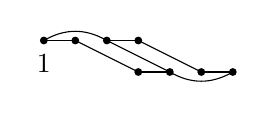
\begin{tikzpicture}[scale=0.4]
\draw[xshift=-1cm] (0,0) node[circle,fill,inner sep=1pt,label=below:$1$]{} -- (1,0)
node[circle,fill,inner sep=1pt]{};
\draw[xshift=-1cm] (2,0) node[circle,fill,inner sep=1pt]{} -- (3,0)
node[circle,fill,inner sep=1pt]{};
\draw[xshift=-1cm] (3,-1) node[circle,fill,inner sep=1pt]{} -- (4,-1)
node[circle,fill,inner sep=1pt]{};
\draw[xshift=-1cm] (5,-1) node[circle,fill,inner sep=1pt]{} -- (6,-1)
node[circle,fill,inner sep=1pt]{};
\draw (-1, 0) to[out=30, in=150] ++(2, 0);
\draw (0,0) to ++(2, -1);
\draw (1,0) to ++(2, -1);
\draw (2,0) to ++(2, -1);
\draw (3,-1) to[out=-30, in=-150] ++(2, 0);
\end{tikzpicture}
}
Each dot represents a class in $A(1)$; lines of horizontal distance 1 represent multiplication by $\mathrm{Sq}^1$, and those of distance 2 represent multiplication by $\mathrm{Sq}^2$.
We will visually construct a free resolution of a single class of $\F_2$ by $A(1)$-modules by ``chasing dots and lines'' exhaustively, killing off all classes that are left over.
In the first step, we map one copy of $A(1)$ to the single copy of $\F_2$:
\marginnote{
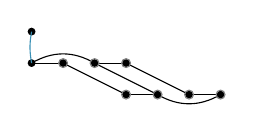
\begin{tikzpicture}[scale=0.4]
\draw (-1, 0) node[circle, fill, inner sep=1pt]{};
\draw[xshift=-1cm, yshift=-1cm] (0,0) node[circle,fill,inner sep=1pt]{} -- (1,0)
node[circle,fill,inner sep=1pt]{};
\draw[xshift=-1cm, yshift = -1cm] (2,0) node[circle,fill,inner sep=1pt]{} -- (3,0)
node[circle,fill,inner sep=1pt]{};
\draw[xshift=-1cm, yshift = -1cm] (3,-1) node[circle,fill,inner sep=1pt]{} -- (4,-1)
node[circle,fill,inner sep=1pt]{};
\draw[xshift=-1cm, yshift = -1cm] (5,-1) node[circle,fill,inner sep=1pt]{} -- (6,-1)
node[circle,fill,inner sep=1pt]{};
\draw[yshift=-1cm] (-1, 0) to[out=30, in=150] ++(2, 0);
\draw[yshift=-1cm] (0,0) to ++(2, -1);
\draw[yshift=-1cm] (1,0) to ++(2, -1);
\draw[yshift=-1cm] (2,0) to ++(2, -1);
\draw[yshift=-1cm] (3,-1) to[out=-30, in=-150] ++(2, 0);
\draw[color = cyan!70!black](-1, -1) to[out=100, in=-100] ++(0, 1);
% circle kernel
\draw[color = gray] (0,-1) circle (4pt);
\draw[color = gray] (1,-1) circle (4pt);
\draw[color = gray] (2,-1) circle (4pt);
\draw[color = gray] (2,-2) circle (4pt);
\draw[color = gray] (3,-2) circle (4pt);
\draw[color = gray] (4,-2) circle (4pt);
\draw[color = gray] (5,-2) circle (4pt);
\end{tikzpicture}
}
The classes not supporting a blue line are in the kernel of this map (circled in gray), and thus survive to the degree one part of the resolution.


Now we turn to resolving the kernel.
The kernel is generated by two classes---namely, the classes with no incoming lines from their left.
Here, the vertical lines are drawn so that the maps are as $A(1)$ modules; i.e., they commute with $\mathrm{Sq}^1$ and $\mathrm{Sq}^2$.
\marginnote{
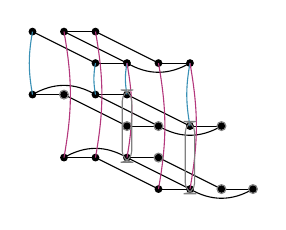
\begin{tikzpicture}[scale=0.4]
\draw (0,0) node[circle,fill,inner sep=1pt]{};
\draw (1,0) node[circle,fill,inner sep=1pt]{} -- (2,0)
node[circle,fill,inner sep=1pt]{};
\draw (2,-1) node[circle,fill,inner sep=1pt]{} -- (3,-1)
node[circle,fill,inner sep=1pt]{};
\draw (4,-1) node[circle,fill,inner sep=1pt]{} -- (5,-1)
node[circle,fill,inner sep=1pt]{};
\draw (0,0) to ++(2, -1);
\draw (1,0) to ++(2, -1);
\draw (2,0) to ++(2, -1);
\draw (3,-1) to[out=-30, in=-150] ++(2, 0);
% copy of A(1) at (0, -2)
\draw (0,-2) node[circle,fill,inner sep=1pt]{} -- (1,-2)
node[circle,fill,inner sep=1pt]{};
\draw (2,-2) node[circle,fill,inner sep=1pt]{} -- (3,-2)
node[circle,fill,inner sep=1pt]{};
\draw (3,-3) node[circle,fill,inner sep=1pt]{} -- (4,-3)
node[circle,fill,inner sep=1pt]{};
\draw (5,-3) node[circle,fill,inner sep=1pt]{} -- (6,-3)
node[circle,fill,inner sep=1pt]{};
\draw (0, -2) to[out=30, in=150] ++(2, 0);
\draw (1,-2) to ++(2, -1);
\draw (2,-2) to ++(2, -1);
\draw (3,-2) to ++(2, -1);
\draw (4,-3) to[out=-30, in=-150] ++(2, 0);
% connecting lines
\draw[color = cyan!70!black] (0, -2) to[out=100, in=-100] ++(0, 2);
\draw[color = cyan!70!black] (2, -2) to[out=100, in=-100] ++(0, 1);
\draw[color = cyan!70!black] (3, -2) to[out=100, in=-100] ++(0, 1);
\draw[color = cyan!70!black] (5, -3) to[out=100, in=-100] ++(0, 2);
% copy of A(1) at (1, -4)
\draw (1,-4) node[circle,fill,inner sep=1pt]{} -- (2,-4)
node[circle,fill,inner sep=1pt]{};
\draw (3,-4) node[circle,fill,inner sep=1pt]{} -- (4,-4)
node[circle,fill,inner sep=1pt]{};
\draw (4,-5) node[circle,fill,inner sep=1pt]{} -- (5,-5)
node[circle,fill,inner sep=1pt]{};
\draw (6,-5) node[circle,fill,inner sep=1pt]{} -- (7,-5) node[circle,fill,inner sep=1pt]{};
\draw (1, -4) to[out=30, in=150] ++(2, 0);
\draw (2,-4) to ++(2, -1);
\draw (3,-4) to ++(2, -1);
\draw (4,-4) to ++(2, -1);
\draw (5,-5) to[out=-30, in=-150] ++(2, 0);
% connecting lines
\draw[color=magenta!70!black] (1, -4) to[out=80, in=-80] ++(0, 4);
\draw[color=magenta!70!black] (2, -4) to[out=80, in=-80] ++(0, 4);
\draw[color=magenta!70!black] (4, -5) to[out=80, in=-80] ++(0, 4);
\draw[color=magenta!70!black] (5, -5) to[out=80, in=-80] ++(0, 4);
\draw[color=magenta!70!black] (3, -4) to[out=80, in=-80] ++(0, 3);
% circle kernel
\draw[color = gray] (1,-2) circle (4pt);
\draw[color = gray] (3,-3) circle (4pt);
\draw[color = gray] (4,-3) circle (4pt);
\draw[color = gray] (6,-3) circle (4pt);
\draw[color = gray] (4,-4) circle (4pt);
\draw[color = gray] (6,-5) circle (4pt);
\draw[color = gray] (7,-5) circle (4pt);
\draw[color = gray, rounded corners = 4pt] (4.85,-2.85) rectangle (5.15, -5.15);
\draw[color = gray, rounded corners = 4pt] (2.85,-1.85) rectangle (3.15, -4.15);
\end{tikzpicture}
}

To move to the next stage of the resolution, we must calculate the kernel at this stage.
If a class supporting a red line and one supporting a blue line both hit the same class, their sum will be in the kernel.
Thus, the diagram to resolve for degree two is as portrayed at right.
\marginnote[-5\baselineskip]{
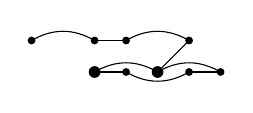
\begin{tikzpicture}[scale=0.4]
% all the dots of kernel
\draw (0,0) node[circle,fill,inner sep=1pt]{};
\draw (2,0) node[circle,fill,inner sep=1pt]{};
\draw (2,-1) node[circle,fill,inner sep=1.5pt]{};
\draw (3,0) node[circle,fill,inner sep=1pt]{};
\draw (3,-1) node[circle,fill,inner sep=1pt]{};
\draw (4,-1) node[circle,fill,inner sep=1.5pt]{};
\draw (5,0) node[circle,fill,inner sep=1pt]{};
\draw (5,-1) node[circle,fill,inner sep=1pt]{};
\draw (6,-1) node[circle,fill,inner sep=1pt]{};
% lines of kernel
\draw (0,0) to[out=30, in=150] ++(2,0);
\draw (2, -1) -- (3, -1);
\draw (2, -1) to[out=30, in=150] ++(2,0);
\draw (4, -1) to[out=30, in=150] ++(2,0);
\draw (2,0) -- (3, 0);
\draw (5,-1) -- (6,-1);
\draw (3,0) to[out=30, in=150] ++(2,0);
\draw (3,-1) to[out=-30, in=-150] ++(2,0);
\draw (4,-1) -- (5, 0);
\end{tikzpicture}
}

Following the same procedure of selecting dots which have no edges incoming from the left, we can produce a surjective map from a free module and hence the next stage of the resolution.
\marginnote{
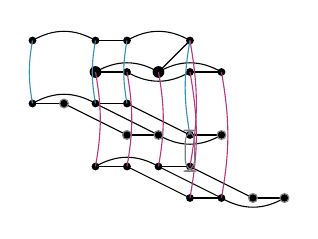
\begin{tikzpicture}[scale=0.4]
% all the dots of kernel
\draw (0,0) node[circle,fill,inner sep=1pt]{};
\draw (2,0) node[circle,fill,inner sep=1pt]{};
\draw (2,-1) node[circle,fill,inner sep=1.5pt]{};
\draw (3,0) node[circle,fill,inner sep=1pt]{};
\draw (3,-1) node[circle,fill,inner sep=1pt]{};
\draw (4,-1) node[circle,fill,inner sep=1.5pt]{};
\draw (5,0) node[circle,fill,inner sep=1pt]{};
\draw (5,-1) node[circle,fill,inner sep=1pt]{};
\draw (6,-1) node[circle,fill,inner sep=1pt]{};
% lines of kernel
\draw (0,0) to[out=30, in=150] ++(2,0);
\draw (2, -1) -- (3, -1);
\draw (2, -1) to[out=30, in=150] ++(2,0);
\draw (4, -1) to[out=30, in=150] ++(2,0);
\draw (2,0) -- (3, 0);
\draw (5,-1) -- (6,-1);
\draw (3,0) to[out=30, in=150] ++(2,0);
\draw (3,-1) to[out=-30, in=-150] ++(2,0);
\draw (4,-1) -- (5, 0);
% copy of A(1) at (0, -2)
\draw (0,-2) node[circle,fill,inner sep=1pt]{} -- (1,-2)
node[circle,fill,inner sep=1pt]{};
\draw (2,-2) node[circle,fill,inner sep=1pt]{} -- (3,-2)
node[circle,fill,inner sep=1pt]{};
\draw (3,-3) node[circle,fill,inner sep=1pt]{} -- (4,-3)
node[circle,fill,inner sep=1pt]{};
\draw (5,-3) node[circle,fill,inner sep=1pt]{} -- (6,-3)
node[circle,fill,inner sep=1pt]{};
\draw (0, -2) to[out=30, in=150] ++(2, 0);
\draw (1,-2) to ++(2, -1);
\draw (2,-2) to ++(2, -1);
\draw (3,-2) to ++(2, -1);
\draw (4,-3) to[out=-30, in=-150] ++(2, 0);
% connecting lines for copy of A(1) at (0, -2)
\draw[color=cyan!70!black] (0,-2) to[out=100, in=-100] ++(0,2);
\draw[color=cyan!70!black] (2,-2) to[out=100, in=-100] ++(0,2);
\draw[color=cyan!70!black] (3,-2) to[out=100, in=-100] ++(0,2);
\draw[color=cyan!70!black] (5,-3) to[out=100, in=-100] ++(0,3);
% copy of A(1) at (2, -4)
\draw (2,-4) node[circle,fill,inner sep=1pt]{} -- (3,-4)
node[circle,fill,inner sep=1pt]{};
\draw (4,-4) node[circle,fill,inner sep=1pt]{} -- (5,-4)
node[circle,fill,inner sep=1pt]{};
\draw (5,-5) node[circle,fill,inner sep=1pt]{} -- (6,-5)
node[circle,fill,inner sep=1pt]{};
\draw (7,-5) node[circle,fill,inner sep=1pt]{} -- (8,-5)
node[circle,fill,inner sep=1pt]{};
\draw (2, -4) to[out=30, in=150] ++(2, 0);
\draw (3,-4) to ++(2, -1);
\draw (4,-4) to ++(2, -1);
\draw (5,-4) to ++(2, -1);
\draw (6,-5) to[out=-30, in=-150] ++(2, 0);
% connecting lines for copy of A(1) at (2, -4)
\draw[color=magenta!70!black] (2,-4) to[out=80, in=-80] ++(0,3);
\draw[color=magenta!70!black] (3,-4) to[out=80, in=-80] ++(0,3);
\draw[color=magenta!70!black] (4,-4) to[out=80, in=-80] ++(0,3);
\draw[color=magenta!70!black] (5,-4) to[out=80, in=-80] ++(0,4);
\draw[color=magenta!70!black] (5,-5) to[out=80, in=-80] ++(0,4);
\draw[color=magenta!70!black] (6,-5) to[out=80, in=-80] ++(0,4);
% circle kernel
\draw[color = gray] (1, -2) circle (4pt);
\draw[color = gray] (3, -3) circle (4pt);
\draw[color = gray] (4, -3) circle (4pt);
\draw[color = gray] (6, -3) circle (4pt);
\draw[color = gray] (7, -5) circle (4pt);
\draw[color = gray] (8, -5) circle (4pt);
\draw[color = gray, rounded corners = 4pt] (4.85,-2.85) rectangle (5.15, -4.15);
\end{tikzpicture}
}

In fact, we have to follow this procedure twice more.
\marginnote{
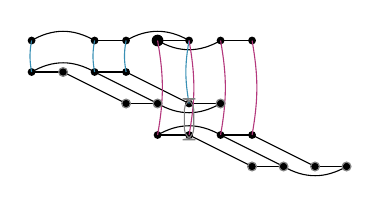
\begin{tikzpicture}[scale=0.4]
% dots of kernel
\draw (0,0) node[circle,fill,inner sep=1pt]{};
\draw (2,0) node[circle,fill,inner sep=1pt]{};
\draw (3,0) node[circle,fill,inner sep=1pt]{};
\draw (4,0) node[circle,fill,inner sep=1.5pt]{};
\draw (5,0) node[circle,fill,inner sep=1pt]{};
\draw (6,0) node[circle,fill,inner sep=1pt]{};
\draw (7,0) node[circle,fill,inner sep=1pt]{};
% lines of kernel
\draw (0,0) to[out=30, in=150] ++(2,0);
\draw (2,0)--(3,0);
\draw (3,0) to[out=30, in=150] ++(2, 0);
\draw (4,0) -- (5, 0);
\draw (4,0) to[out=-30, in=-150] ++(2,0);
\draw (6,0) -- (7,0);
% copy of A(1) at (0,-1)
\draw (0,-1) node[circle,fill,inner sep=1pt]{} -- (1,-1)
node[circle,fill,inner sep=1pt]{};
\draw (2,-1) node[circle,fill,inner sep=1pt]{} -- (3,-1)
node[circle,fill,inner sep=1pt]{};
\draw (3,-2) node[circle,fill,inner sep=1pt]{} -- (4,-2)
node[circle,fill,inner sep=1pt]{};
\draw (5,-2) node[circle,fill,inner sep=1pt]{} -- (6,-2)
node[circle,fill,inner sep=1pt]{};
\draw (0, -1) to[out=30, in=150] ++(2, 0);
\draw (1,-1) to ++(2, -1);
\draw (2,-1) to ++(2, -1);
\draw (3,-1) to ++(2, -1);
\draw (4,-2) to[out=-30, in=-150] ++(2, 0);
% connecting lines for copy of A(1) at (0, -1)
\draw[color=cyan!70!black] (0,-1) to[out=100, in=-100] ++(0,1);
\draw[color=cyan!70!black] (2,-1) to[out=100, in=-100] ++(0,1);
\draw[color=cyan!70!black] (3,-1) to[out=100, in=-100] ++(0,1);
\draw[color=cyan!70!black] (5,-2) to[out=100, in=-100] ++(0,2);
% copy of A(1) at (4,-3)
\draw (4,-3) node[circle,fill,inner sep=1pt]{} -- (5,-3)
node[circle,fill,inner sep=1pt]{};
\draw (6,-3) node[circle,fill,inner sep=1pt]{} -- (7,-3)
node[circle,fill,inner sep=1pt]{};
\draw (7,-4) node[circle,fill,inner sep=1pt]{} -- (8,-4)
node[circle,fill,inner sep=1pt]{};
\draw (9,-4) node[circle,fill,inner sep=1pt]{} -- (10,-4)
node[circle,fill,inner sep=1pt]{};
\draw (4, -3) to[out=30, in=150] ++(2, 0);
\draw (5,-3) to ++(2, -1);
\draw (6,-3) to ++(2, -1);
\draw (7,-3) to ++(2, -1);
\draw (8,-4) to[out=-30, in=-150] ++(2, 0);
% connecting lines for copy of A(1) at (4,-3)
\draw[color=magenta!70!black] (4,-3) to[out=80, in=-80] ++(0,3);
\draw[color=magenta!70!black] (5,-3) to[out=80, in=-80] ++(0,3);
\draw[color=magenta!70!black] (6,-3) to[out=80, in=-80] ++(0,3);
\draw[color=magenta!70!black] (7,-3) to[out=80, in=-80] ++(0,3);
% circle kernel
\draw[color = gray] (1, -1) circle (4pt);
\draw[color = gray] (3, -2) circle (4pt);
\draw[color = gray] (4, -2) circle (4pt);
\draw[color = gray] (6, -2) circle (4pt);
\draw[color = gray] (7, -4) circle (4pt);
\draw[color = gray] (8, -4) circle (4pt);
\draw[color = gray] (9, -4) circle (4pt);
\draw[color = gray] (10, -4) circle (4pt);
\draw[color = gray, rounded corners = 4pt] (4.85,-1.85) rectangle (5.15, -3.15);
\end{tikzpicture}
}
\todo{This is missing the gray circles.}
\marginnote{
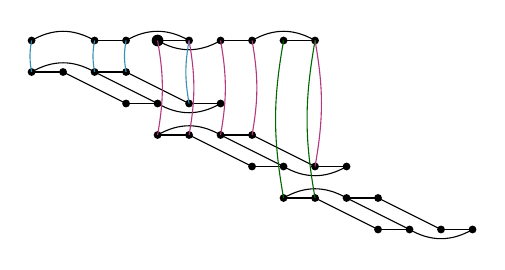
\begin{tikzpicture}[scale=0.4]
% dots of kernel
\draw (0,0) node[circle,fill,inner sep=1pt]{};
\draw (2,0) node[circle,fill,inner sep=1pt]{};
\draw (3,0) node[circle,fill,inner sep=1pt]{};
\draw (4,0) node[circle,fill,inner sep=1.5pt]{};
\draw (5,0) node[circle,fill,inner sep=1pt]{};
\draw (6,0) node[circle,fill,inner sep=1pt]{};
\draw (7,0) node[circle,fill,inner sep=1pt]{};
\draw (8,0) node[circle,fill,inner sep=1pt]{};
\draw (9,0) node[circle,fill,inner sep=1pt]{};
% lines of kernel
\draw (0,0) to[out=30, in=150] ++(2,0);
\draw (2,0)--(3,0);
\draw (3,0) to[out=30, in=150] ++(2, 0);
\draw (4,0) -- (5, 0);
\draw (4,0) to[out=-30, in=-150] ++(2,0);
\draw (6,0) -- (7,0);
\draw (7,0) to[out=30, in=150] ++(2,0);
\draw (8,0) -- (9,0);
% copy of A(1) at (0, -1)
\draw (0,-1) node[circle,fill,inner sep=1pt]{} -- (1,-1)
node[circle,fill,inner sep=1pt]{};
\draw (2,-1) node[circle,fill,inner sep=1pt]{} -- (3,-1)
node[circle,fill,inner sep=1pt]{};
\draw (3,-2) node[circle,fill,inner sep=1pt]{} -- (4,-2)
node[circle,fill,inner sep=1pt]{};
\draw (5,-2) node[circle,fill,inner sep=1pt]{} -- (6,-2)
node[circle,fill,inner sep=1pt]{};
\draw (0, -1) to[out=30, in=150] ++(2, 0);
\draw (1,-1) to ++(2, -1);
\draw (2,-1) to ++(2, -1);
\draw (3,-1) to ++(2, -1);
\draw (4,-2) to[out=-30, in=-150] ++(2, 0);
% connecting lines for copy of A(1) at (0, -1)
\draw[color=cyan!70!black] (0,-1) to[out=100, in=-100] ++(0,1);
\draw[color=cyan!70!black] (2,-1) to[out=100, in=-100] ++(0,1);
\draw[color=cyan!70!black] (3,-1) to[out=100, in=-100] ++(0,1);
\draw[color=cyan!70!black] (5,-2) to[out=100, in=-100] ++(0,2);
% copy of A(1) at (4,-3)
\draw (4,-3) node[circle,fill,inner sep=1pt]{} -- (5,-3)
node[circle,fill,inner sep=1pt]{};
\draw (6,-3) node[circle,fill,inner sep=1pt]{} -- (7,-3)
node[circle,fill,inner sep=1pt]{};
\draw (7,-4) node[circle,fill,inner sep=1pt]{} -- (8,-4)
node[circle,fill,inner sep=1pt]{};
\draw (9,-4) node[circle,fill,inner sep=1pt]{} -- (10,-4)
node[circle,fill,inner sep=1pt]{};
\draw (4, -3) to[out=30, in=150] ++(2, 0);
\draw (5,-3) to ++(2, -1);
\draw (6,-3) to ++(2, -1);
\draw (7,-3) to ++(2, -1);
\draw (8,-4) to[out=-30, in=-150] ++(2, 0);
% connecting lines for copy of A(1) at (4,-3)
\draw[color=magenta!70!black] (4,-3) to[out=80, in=-80] ++(0,3);
\draw[color=magenta!70!black] (5,-3) to[out=80, in=-80] ++(0,3);
\draw[color=magenta!70!black] (6,-3) to[out=80, in=-80] ++(0,3);
\draw[color=magenta!70!black] (7,-3) to[out=80, in=-80] ++(0,3);
\draw[color=magenta!70!black] (9,-4) to[out=80, in=-80] ++(0,4);
% copy of A(1) at (8, -5)
\draw (8,-5) node[circle,fill,inner sep=1pt]{} -- (9,-5)
node[circle,fill,inner sep=1pt]{};
\draw (10,-5) node[circle,fill,inner sep=1pt]{} -- (11,-5)
node[circle,fill,inner sep=1pt]{};
\draw (11,-6) node[circle,fill,inner sep=1pt]{} -- (12,-6)
node[circle,fill,inner sep=1pt]{};
\draw (13,-6) node[circle,fill,inner sep=1pt]{} -- (14,-6)
node[circle,fill,inner sep=1pt]{};
\draw (8, -5) to[out=30, in=150] ++(2, 0);
\draw (9,-5) to ++(2, -1);
\draw (10,-5) to ++(2, -1);
\draw (11,-5) to ++(2, -1);
\draw (12,-6) to[out=-30, in=-150] ++(2, 0);
% connecting lines for copy of A(1) at (8, -5)
\draw[color=green!40!black] (8,-5) to[out=100, in=-100] ++(0,5);
\draw[color=green!40!black] (9,-5) to[out=100, in=-100] ++(0,5);
\end{tikzpicture}
}
Note that this kernel decomposes into a sum of modules, each of which we've seen before.
\todo[inline]{Draw this kernel, gives names to the summands.}
We can use this observation to extend this to an infinite free resolution by appropriately repeating the steps we have already taken.
Since the cohomology of the cobar complex is meant to compute $\Ext_{\A(1)_*}^{*, *}(\F_2, \F_2)$, we can equivalently compute its cohomology by mapping our minimal free resolution into $\F_2$ and calculating its cohomology---which carries the trivial differential.
In all, this produces the family of $\Ext$--groups pictured at right.
\marginnote{%
\begin{sseqdata}[ name = A1ExtGroups ]
\class(0,0)
\foreach \y in {1,...,9} { \class(0, \y) \structline }
\class(1,1)
\class(2,2)

\class(4,3)
\foreach \y in {4,...,9} { \class(4, \y) \structline }

\class(8,5)
\foreach \y in {6,...,9} { \class(8, \y) \structline }
\class(9,6)
\class(10,7)
\end{sseqdata}
\printpage[ name = A1ExtGroups, x range = {0}{10}, y range = {0}{8}, yscale = 0.3, xscale = 0.3 ]
}

Now we consider a less manual method of computing these $\Ext$ groups.
We will need a filtration to produce a spectral sequence, and we select the filtration given by powers of the augmentation ideal.
This is a useful choice because the associated graded looks like the cobar complex for an exterior algebra, which has known homology: it is given by a polynomial algebra on homology-suspended shifts of the same classes.

\begin{theorem}[May]\marginnote{\citep{May}}
This gives a spectral sequence of algebras \[E_1^{*, *, *} \cong \F_2[h_{10}, h_{11}, h_{20}] \Rightarrow H^*(\A(1)_*),\] where $h_{ij}$ represents $\xi_i^{2^j}$. \qed
\end{theorem}

The first differential in this spectral sequence is tautological to compute:

\begin{lemma}
$d_1$ is fully specified by
\begin{align*}
d_1(h_{10}) & = 0, &
d_1(h_{11}) & = 0, &
d_1(h_{20}) & = h_{10} h_{11}.
\end{align*}
\end{lemma}
\begin{proof}
Recall that $h_{ij}$ represents $\xi_i^{2^j}$.
The first two equations then follow from $\delta^1(\xi_1^{2^j}) = 0$.
To analyze $h_{20}$, note that the differential of $\xi_2$ in the cobar complex is \[\delta^1(\xi_2) = \Delta \xi_2 = \xi_1 \mid \xi_1^2.\]
This is represented by $h_{10} h_{11}$.
\end{proof}

\noindent
\marginnote{%
\DeclareSseqGroup\hzerotower {} {\foreach \y in {1,...,9} { \class(0,\y) }}
\DeclareSseqGroup\honetower  {} {\foreach \y in {1,...,9} { \class(\y,\y) }}
\DeclareSseqGroup\AOneWing {} {
    \class(0,0)
    \foreach \y in {1,...,9} { \class(0, \y) \structline }
    \class(1,1) \structline(0,0)(1,1)
    \foreach \y in {2,...,9} { \class(\y, \y) \structline }
}
\begin{sseqdata}[ name = MaySSA1, yscale = 0.3, xscale = 0.3 ]
\AOneWing(0,0)
\AOneWing(4,2)
\AOneWing(8,4)
\AOneWing(12,6)
\end{sseqdata}
\printpage[ name = MaySSA1, page = 2, x range = {0}{10}, y range = {0}{8} ] \\
Vertical lines indicate classes linked by multiplication by $h_{10}$, and diagonal lines indicate classes linked by multiplication by $h_{11}$.
}
Since these form a multiplicative generating set, we can use the Leibniz law to capture the rest of $d_1$: \[d_1(x y) = (d_1 x) y + (-1)^{|x|} x (d_1 y).\]

\begin{lemma}
$d(h_{20}^2) = h_{11}^3$.
\end{lemma}
\begin{proof}
The class $h_{20}^2$ is represented by $\xi_2 \mid \xi_2$, which has cobar differential \[\delta(\xi_2 \mid \xi_2) = \xi_1 \mid \xi_1^2 \mid \xi_2 + \xi_2 \mid \xi_1 \mid \xi_1^2,\] which in turn represents \[2 h_{10} h_{11} h_{20} \equiv 0.\]
That this class vanishes in the spectral sequence indicates that we can produce a longer spectral sequence differential by adding a correcting term of higher filtration to the chosen representative $\xi_2 \mid \xi_2$.
Namely, we need to find a preimage of $\xi_1 \mid \xi_1^2 \mid \xi_2 + \xi_2 \mid \xi_1 \mid \xi_1^2$ along the cobar differential, up to higher still filtration.
Some fussing shows that the following fits the bill: \[\xi_1 \xi_2 \mid \xi_1^2 + \xi_1 \mid \xi_2 \xi_1^2,\] from which we compute
\begin{align*}
d(\xi_2 \mid \xi_2 + \xi_1 \xi_2 \mid \xi_1^2 + \xi_1 \mid \xi_2 \xi_1^2)
&       = (\xi_1 \mid \xi_1^2 \mid \xi_2 + \xi_2 \mid \xi_1 \mid \xi_1^2) \\
& \quad + (\xi_1^2 \mid \xi_1^2 + \xi_1 \mid \xi_2 + \xi_2 \mid \xi_1 + \xi_1 \mid \xi_1^3) \mid \xi_1^2 \\
& \quad + \xi_1 \mid (\xi_2 \mid \xi_1^2 + \xi_1 \mid \xi_1^4 + \xi_1^2 \mid \xi_2 + \xi_1^3 \mid \xi_1^2) \\
& = \xi_1^2 \mid \xi_1^2 \mid \xi_1^2.
\end{align*}
This last class represents $h_{11}^3$, which is nonzero on the second page of the May spectral sequence.
\end{proof}

\noindent
\marginnote{%
\begin{sseqdata}[ name = MaySSA1, update existing ]
\foreach \j in {0,...,6} {
    \d2(4+\j,2+\j)(3+\j,3+\j)
}
\foreach \j in {0,...,6} {
    \d2(12+\j,6+\j)(11+\j,7+\j)
}
\end{sseqdata}
\printpage[ name = MaySSA1, page = 3, x range = {0}{10}, y range = {0}{8} ]
}
This again is enough to determine the differential on a multiplicative generating set.
More than this, this is the last differential in the spectral sequence, since the page is now too sparse to support any further differentials.
In this way, the spectral sequence and its multiplicative structure have converted the computation the cohomology of an infinite complex, a seemingly intractible problem, into two relatively minor calculations in the complex.

\begin{remark}
\todo[inline]{Expand remark about Leibniz rule into the Christianson-style presentation of the spectral sequence.}
\end{remark}

% We'll talk about this smaller example in a language that generalizes.  The specification of the spectral sequence above is multiplicative, in the sense that the Leibniz rule specifies everything.  Computation can be made \emph{linear} again by working with $E_1^2 = \F_2[h_{10}^2, h_{11}^2, h_{20}^2]$--modules.
% \[
% \begin{array}{c|cccccccc}
% d_1 & 1 & h_{10} & h_{11} & h_{20} & h_{10} h_{11} & h_{11} h_{20} & h_{10} h_{20} & h_{10} h_{11} h_{20} \\
% \hline
% 1                    & 0 & 0 & 0 & 0 & 0 &        0 &        0 & h_{10}^2 h_{11}^2 \\
% h_{10}               & 0 & 0 & 0 & 0 & 0 & h_{11}^2 &        0 & 0 \\
% h_{11}               & 0 & 0 & 0 & 0 & 0 &        0 & h_{10}^2 & 0 \\
% h_{20}               & 0 & 0 & 0 & 0 & 0 &        0 &        0 & 0 \\
% h_{10} h_{11}        & 0 & 0 & 0 & 1 & 0 &        0 &        0 & 0 \\
% h_{11} h_{20}        & 0 & 0 & 0 & 0 & 0 &        0 &        0 & 0 \\
% h_{10} h_{20}        & 0 & 0 & 0 & 0 & 0 &        0 &        0 & 0 \\
% h_{10} h_{11} h_{20} & 0 & 0 & 0 & 0 & 0 &        0 &        0 & 0
% \end{array},
% \]
% hence $Z = E_1^2\{1, h_{10}, h_{11}, h_{10} h_{11}\}$ and $B = \<1 \cdot h_{10} h_{11}, h_{11}^2 \cdot h_{10}, h_{10}^2 \cdot h_{11}, h_{10}^2 h_{11}^2 \cdot 1\>$, from which we see \[E_2 = H = E_1^2\{1 / h_{10}^2 h_{11}^2, h_{10} / h_{11}^2, h_{11} / h_{10}^2\}.\]\todo{include picture}

% To continue the calculation, we need some way to describe longer differentials in the spectral sequence.

% \begin{theorem}[Nakamura]
% There are operators $\Sq^n$ acting on the May spectral sequence, satisfying\ldots
% \begin{enumerate}
%     \item $\Sq^0 h_{ij} = h_{i(j+1)}$.
%     \item $\Sq^1 h_{ij} = h_{ij}^2$.
%     \item $\Sq^n$ is linear.
%     \item $\Sq^n(x \cdot y) = \sum_{i+j=n} \Sq^i(x) \Sq^j(y)$.
%     \item $\Sq^n(d_? x) = d_? \Sq^n(x)$, where ``$?$'' is \emph{unknown}.
% \end{enumerate}
% \end{theorem}

% \begin{example}
% \[d_?(h_{20}^2) = d_?(\Sq^1 h_{20}) = \Sq^1 d_1 h_{20} = \Sq^1(h_{10} h_{11}) = \Sq^1 h_{10} \Sq^0 h_{11} + \Sq^0 h_{10} \Sq^1 h_{11} = h_{10}^2 h_{12} + h_{11}^3.\]
% \end{example}

% We compute the subalgebra of squares to be $E_2^2 = \F_2[h_{10}^4, h_{11}^2, h_{20}^4] / (h_{10}^2 h_{11}^2)$, and continuing in this way gives a computation of $d_2$ as an $E_2^2$--linear map.
% \[
% \begin{array}{c|cccccc}
% d_2 & 1 & h_{10}/h_{11}^2 & h_{11}/h_{10}^2 & h_{10}h_{20}^2/h_{11}^2 & h_{11}h_{20}^2/h_{10}^2 & h_{20}^2 \\
% 1 &                       0 & 0 & 0 & 0 & h_{11}^4 & 0 \\
% h_{10}/h_{11}^2 &         0 & 0 & 0 & 0 &        0 & 0 \\
% h_{11}/h_{10}^2 &         0 & 0 & 0 & 0 &        0 & h_{11}^2 \\
% h_{10}h_{20}^2/h_{11}^2 & 0 & 0 & 0 & 0 &        0 & 0 \\
% h_{11}h_{20}^2/h_{10}^2 & 0 & 0 & 0 & 0 &        0 & 0 \\
% h_{20}^2                & 0 & 0 & 0 & 0 &        0 & 0               
% \end{array}
% \]
% This has kernel $Z = \<1, h_{10}, h_{11}, h_{10}h_{20}^2, h_{10}^2h_{20}^2\>$ and image $B = \<h_{11}^4 \cdot 1, h_{11}^2 \cdot h_{11}\>$, hence cohomology \[E_3 = H = E_2^2\{1 / h_{11}^4, h_{10}/h_{11}^2, h_{11} / (h_{10}^2, h_{11}^2), h_{10}h_{20}^2/h_{11}^2, h_{10}^2h_{20}^2 / h_{11}^2\}.\]  This is the last page; we include a sketch below.\todo{sketch}

% The general computation is similar in techniques, but vastly more complicated.  (For $\A(2)$, it still turns out to be completely feasible, and was first worked in (I think...!) by Mahowald and Hopkins.)






\end{subappendices}





